% Options for packages loaded elsewhere
\PassOptionsToPackage{unicode}{hyperref}
\PassOptionsToPackage{hyphens}{url}
\PassOptionsToPackage{dvipsnames,svgnames,x11names}{xcolor}
%
\documentclass[
]{article}
\usepackage{amsmath,amssymb}
\usepackage{iftex}
\ifPDFTeX
  \usepackage[T1]{fontenc}
  \usepackage[utf8]{inputenc}
  \usepackage{textcomp} % provide euro and other symbols
\else % if luatex or xetex
  \usepackage{unicode-math} % this also loads fontspec
  \defaultfontfeatures{Scale=MatchLowercase}
  \defaultfontfeatures[\rmfamily]{Ligatures=TeX,Scale=1}
\fi
\usepackage{lmodern}
\ifPDFTeX\else
  % xetex/luatex font selection
\fi
% Use upquote if available, for straight quotes in verbatim environments
\IfFileExists{upquote.sty}{\usepackage{upquote}}{}
\IfFileExists{microtype.sty}{% use microtype if available
  \usepackage[]{microtype}
  \UseMicrotypeSet[protrusion]{basicmath} % disable protrusion for tt fonts
}{}
\makeatletter
\@ifundefined{KOMAClassName}{% if non-KOMA class
  \IfFileExists{parskip.sty}{%
    \usepackage{parskip}
  }{% else
    \setlength{\parindent}{0pt}
    \setlength{\parskip}{6pt plus 2pt minus 1pt}}
}{% if KOMA class
  \KOMAoptions{parskip=half}}
\makeatother
\usepackage{xcolor}
\usepackage[margin=1in]{geometry}
\usepackage{graphicx}
\makeatletter
\def\maxwidth{\ifdim\Gin@nat@width>\linewidth\linewidth\else\Gin@nat@width\fi}
\def\maxheight{\ifdim\Gin@nat@height>\textheight\textheight\else\Gin@nat@height\fi}
\makeatother
% Scale images if necessary, so that they will not overflow the page
% margins by default, and it is still possible to overwrite the defaults
% using explicit options in \includegraphics[width, height, ...]{}
\setkeys{Gin}{width=\maxwidth,height=\maxheight,keepaspectratio}
% Set default figure placement to htbp
\makeatletter
\def\fps@figure{htbp}
\makeatother
\setlength{\emergencystretch}{3em} % prevent overfull lines
\providecommand{\tightlist}{%
  \setlength{\itemsep}{0pt}\setlength{\parskip}{0pt}}
\setcounter{secnumdepth}{-\maxdimen} % remove section numbering
\usepackage{float}
\usepackage{multirow}
\usepackage{booktabs}
\usepackage{caption}
\usepackage{longtable}
\usepackage{colortbl}
\usepackage{array}
\usepackage{anyfontsize}
\usepackage{multirow}
\ifLuaTeX
  \usepackage{selnolig}  % disable illegal ligatures
\fi
\usepackage{bookmark}
\IfFileExists{xurl.sty}{\usepackage{xurl}}{} % add URL line breaks if available
\urlstyle{same}
\hypersetup{
  pdftitle={Homework 1},
  colorlinks=true,
  linkcolor={Maroon},
  filecolor={Maroon},
  citecolor={Blue},
  urlcolor={blue},
  pdfcreator={LaTeX via pandoc}}

\title{Homework 1}
\author{}
\date{\vspace{-2.5em}}

\begin{document}
\maketitle

\subsubsection{Problem 1.1 ADEMP
Structure}\label{problem-1.1-ademp-structure}

Answer the following questions:

\begin{itemize}
\tightlist
\item
  How many simulation scenarios will you be running?
\end{itemize}

18 scenarios.

\begin{itemize}
\tightlist
\item
  What are the estimand(s)
\end{itemize}

The average treatment effect (\(\beta_{treatment}\))

\begin{itemize}
\tightlist
\item
  What method(s) are being evaluated/compared?
\end{itemize}

The study evaluates the multiple linear regression model and compares
three methods for constructing confidence intervals: 1) Wald confidence
intervals; 2) nonparametric bootstrap percentile intervals; 3)
nonparametric bootstrap-t intervals.

\begin{itemize}
\tightlist
\item
  What are the performance measure(s)?

  \begin{itemize}
  \tightlist
  \item
    Bias of \(\hat{\beta}\)
  \item
    Coverage of \(\hat{\beta}\)
  \item
    Distribution of \(se(\hat{\beta})\)
  \item
    Computation time across methods
  \end{itemize}
\end{itemize}

\subsubsection{Problem 1.2 nSim}\label{problem-1.2-nsim}

Based on desired coverage of 95\% with Monte Carlo error of no more than
1\%, how many simulations (\(n_{sim}\)) should we perform for each
simulation scenario? Implement this number of simulations throughout
your simulation study.

We should perform 475 simulations for each scenario.

\subsubsection{Problem 1.3
Implementation}\label{problem-1.3-implementation}

\subsubsection{Problem 1.4 Results
summary}\label{problem-1.4-results-summary}

\paragraph{\texorpdfstring{Bias of
\(\hat{\beta}\)}{Bias of \textbackslash hat\{\textbackslash beta\}}}\label{bias-of-hatbeta}

\begin{table}[!t]
\caption*{
{\large Average Bias of \(\hat{\beta}\) Across 475 Simulations}
} 
\fontsize{12.0pt}{14.4pt}\selectfont
\begin{tabular*}{\linewidth}{@{\extracolsep{\fill}}ccccccccc}
\toprule
\multicolumn{3}{c}{n = 10} & \multicolumn{3}{c}{n = 50} & \multicolumn{3}{c}{n = 500} \\ 
\cmidrule(lr){1-3} \cmidrule(lr){4-6} \cmidrule(lr){7-9}
\(\beta\) = 0 & \(\beta\) = 0.5 & \(\beta\) = 2 & \(\beta\) = 0 & \(\beta\) = 0.5 & \(\beta\) = 2 & \(\beta\) = 0 & \(\beta\) = 0.5 & \(\beta\) = 2 \\ 
\midrule\addlinespace[2.5pt]
\multicolumn{9}{l}{normal} \\[2.5pt] 
\midrule\addlinespace[2.5pt]
0.015 & 0.040 & 0.011 & 0.021 & -0.007 & -0.013 & 0.002 & -0.006 & -0.004 \\ 
\midrule\addlinespace[2.5pt]
\multicolumn{9}{l}{lognormal} \\[2.5pt] 
\midrule\addlinespace[2.5pt]
0.176 & -0.209 & -0.195 & 0.090 & -0.002 & 0.155 & -0.011 & -0.040 & -0.006 \\ 
\bottomrule
\end{tabular*}
\end{table}

\paragraph{\texorpdfstring{Coverage of
\(\hat{\beta}\)}{Coverage of \textbackslash hat\{\textbackslash beta\}}}\label{coverage-of-hatbeta}

\begin{table}[!t]
\caption*{
{\large Average Coverage of 95\% Wald, Percentile \& Bootstrap-t CIs}
} 
\fontsize{12.0pt}{14.4pt}\selectfont
\begin{tabular*}{\linewidth}{@{\extracolsep{\fill}}crrrrr}
\toprule
family & n & beta\_true & coverage\_wald & coverage\_percentile & coverage\_t \\ 
\midrule\addlinespace[2.5pt]
normal & 10 & 0.0 & 0.926 & 0.848 & 0.945 \\ 
normal & 10 & 0.5 & 0.951 & 0.869 & 0.976 \\ 
normal & 10 & 2.0 & 0.957 & 0.906 & 0.974 \\ 
normal & 50 & 0.0 & 0.926 & 0.926 & 0.931 \\ 
normal & 50 & 0.5 & 0.945 & 0.933 & 0.941 \\ 
normal & 50 & 2.0 & 0.922 & 0.912 & 0.926 \\ 
normal & 500 & 0.0 & 0.954 & 0.954 & 0.945 \\ 
normal & 500 & 0.5 & 0.939 & 0.943 & 0.937 \\ 
normal & 500 & 2.0 & 0.935 & 0.933 & 0.926 \\ 
lognormal & 10 & 0.0 & 0.977 & 0.861 & 0.936 \\ 
lognormal & 10 & 0.5 & 0.951 & 0.844 & 0.960 \\ 
lognormal & 10 & 2.0 & 0.964 & 0.864 & 0.943 \\ 
lognormal & 50 & 0.0 & 0.964 & 0.924 & 0.897 \\ 
lognormal & 50 & 0.5 & 0.964 & 0.912 & 0.884 \\ 
lognormal & 50 & 2.0 & 0.966 & 0.924 & 0.891 \\ 
lognormal & 500 & 0.0 & 0.973 & 0.949 & 0.924 \\ 
lognormal & 500 & 0.5 & 0.966 & 0.949 & 0.933 \\ 
lognormal & 500 & 2.0 & 0.985 & 0.966 & 0.941 \\ 
\bottomrule
\end{tabular*}
\end{table}

\paragraph{\texorpdfstring{Distribution of
\(se(\hat{\beta})\)}{Distribution of se(\textbackslash hat\{\textbackslash beta\})}}\label{distribution-of-sehatbeta}

\begin{center}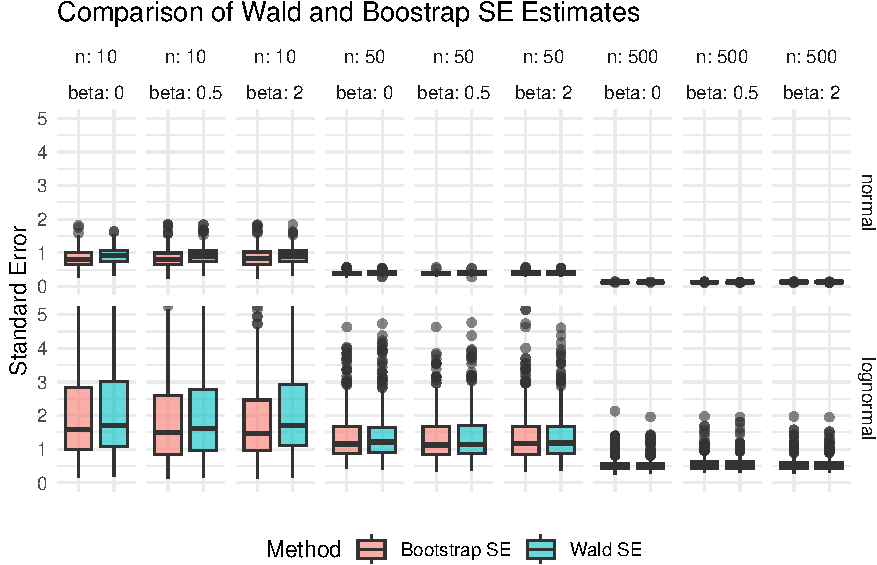
\includegraphics[width=1\linewidth]{HW1_report_files/figure-latex/unnamed-chunk-5-1} \end{center}

\subsubsection{Computation time across
methods}\label{computation-time-across-methods}

\begin{table}[!t]
\caption*{
{\large Average Computation Time for Wald, Percentile \& Bootstrap-t CIs}
} 
\fontsize{12.0pt}{14.4pt}\selectfont
\begin{tabular*}{\linewidth}{@{\extracolsep{\fill}}crrrrr}
\toprule
family & n & beta\_true & time\_wald & time\_percentile & time\_t \\ 
\midrule\addlinespace[2.5pt]
normal & 10 & 0.0 & 0.007 & 0.505 & 169.902 \\ 
normal & 10 & 0.5 & 0.007 & 0.509 & 166.921 \\ 
normal & 10 & 2.0 & 0.008 & 0.529 & 168.568 \\ 
normal & 50 & 0.0 & 0.007 & 0.517 & 173.953 \\ 
normal & 50 & 0.5 & 0.007 & 0.515 & 173.625 \\ 
normal & 50 & 2.0 & 0.007 & 0.516 & 174.564 \\ 
normal & 500 & 0.0 & 0.007 & 0.544 & 200.597 \\ 
normal & 500 & 0.5 & 0.007 & 0.553 & 199.982 \\ 
normal & 500 & 2.0 & 0.007 & 0.554 & 199.987 \\ 
lognormal & 10 & 0.0 & 0.007 & 0.496 & 168.355 \\ 
lognormal & 10 & 0.5 & 0.006 & 0.411 & 143.714 \\ 
lognormal & 10 & 2.0 & 0.006 & 0.441 & 151.516 \\ 
lognormal & 50 & 0.0 & 0.006 & 0.444 & 155.849 \\ 
lognormal & 50 & 0.5 & 0.006 & 0.456 & 156.557 \\ 
lognormal & 50 & 2.0 & 0.006 & 0.446 & 156.140 \\ 
lognormal & 500 & 0.0 & 0.006 & 0.489 & 180.460 \\ 
lognormal & 500 & 0.5 & 0.006 & 0.476 & 179.873 \\ 
lognormal & 500 & 2.0 & 0.006 & 0.479 & 180.365 \\ 
\bottomrule
\end{tabular*}
\end{table}

\subsubsection{Problem 1.5 Discussion}\label{problem-1.5-discussion}

Summary of main findings:

The bias of \(\hat{\beta}\) decreases as the sample size (n) increases.
In small samples (n = 10 or 50), misspecifying the error distribution
leads to biased estimates when the true error distribution is lognormal,
but this bias diminishes in larger samples (n = 500). The Wald
confidence interval maintains coverage near its nominal level (95\%)
when the error distribution is normal and slightly exceeds it when the
true distribution is lognormal, likely due to conservative standard
error (SE) estimates under misspecification. The bootstrap percentile
interval performs poorly in small samples (n = 10) but improves with
increasing n.~In contrast, the bootstrap-t interval performs well in
small samples but does not improve with larger n.~SE estimates from the
Wald and bootstrap methods are similar, with bootstrap estimates
slightly higher. Under model misspecification, SE estimates exhibit
greater variance and right skewness. The variance of SE estimates
decreases as n increases. Regarding computation time, the Wald method is
the fastest, followed by the percentile method, while the bootstrap-t
method is significantly more computationally intensive. No clear trend
is observed in bias, coverage, SE, or computation time across different
true \(\beta\) values.

\begin{itemize}
\tightlist
\item
  Regarding computation time, the Wald method is the fastest, followed
  by the percentile method, while the bootstrap-t method is
  significantly more computationally intensive.
\item
  The bootstrap-t method for constructing confidence intervals provide
  the best coverage when \(\epsilon_i \sim N(0, 2)\).
\item
  The Wald method for constructing confidence intervals provide the best
  coverage when \(\epsilon_i \sim logNormal(0, \log (2))\).
\end{itemize}

\end{document}
